\section{Complexity Theory} \label{sec:6}

\subsection{The Complexity Class $\Poly$} \label{subsec:6.1}
The complexity class $\Poly$ consists of all problems that can be solved
efficiently (in polynomial time). 
\begin{itemize}
    \item The problem $\textsc{MST}$ of finding a minimum spanning tree is in $\Poly$ 
    using Prim's or Kruskal's algorithm. 
    \item The problem $\textsc{ShortestPaths}$ is in $\Poly$ using Dijkstra's algorithm.
    \item The problem $\textsc{MCA}$ of finding a minimum cost arborescence is in 
    $\Poly$ by using Edmonds' algorithm. 
    \item However, we are unsure whether or not $\textsc{MSteinerT}$ and $\textsc{MMSteinerT}$
    are in $\Poly$. We'll discuss this further when we introduce the class $\NP$.
\end{itemize}

Let $X$ be a minimization problem. The {\bf decision problem} corresponding 
to $X$ takes as input an instance of $X$ and a number $k$, and answers 
if there is a feasible solution for the given instance of value at most $k$. 

For example, the decision version of the $\textsc{MSteinerT}$ problem, 
which we'll call $\textsc{DecisionMSteinerT}$, takes as input a graph 
$G = (V, E)$, costs $c_e \geq 0$ for $e \in E$, terminals $T \subseteq V$, 
and a number $k$. To solve the problem, we should output ``yes'' if there 
exists a Steiner tree of cost at most $k$, and output ``no'' otherwise. 

We'll be working with linear programs a lot later in this course. Therefore, 
we should note that solving a linear program is in $\Poly$. 
\begin{itemize}
    \item It is still not known whether the simplex algorithm can be implemented 
    to give a polynomial running time in the worst case. The hard part is the choice of 
    the pivoting rule; it is known that Bland's rule, which ensures that 
    the simplex algorithm never cycles, is quite inefficient.
    \item There are other algorithms that can solve linear programs in 
    polynomial time. The first one to be discovered was the ellipsoid method, 
    but it is also inefficient in practice. 
\end{itemize} 

\subsection{Polynomial Time Reductions} \label{subsec:6.2}
We have seen a glimpse of reductions when we discussed 
$\textsc{MSteinerT}$ and $\textsc{MMSteinerT}$ in Section~\ref{subsec:5.2}. 
Given two problems $X$ and $Y$, we say that $X$ {\bf reduces} in polynomial 
time to $Y$, denoted by $X \leq_P Y$, if one can solve $X$ by using a 
polynomial number of basic operations and a polynomial number of calls 
to an oracle that solves $Y$. Intuitively, this means that $X$ is ``not 
harder'' than $Y$, because if we know how to solve $Y$, then we have 
a way to solve $X$. We look at some examples of reductions.
\begin{itemize}
    \item We can show that $\textsc{MST} \leq_P \textsc{MSteinerT}$. 
    Suppose we are given an instance of $\textsc{MST}$, namely a graph 
    $G = (V, E)$ and edge costs $c_e$ for each $e \in E$. Then we can 
    construct an instance of $\textsc{MSteinerT}$ by simply setting 
    $T = V$. We can pass $(G, c, T)$ to an oracle that solves $\textsc{MSteinerT}$
    and output that result. 
    Overall, this process involved a polynomial number of operations 
    (assigning $T = V$), and then a polynomial number of calls to 
    the oracle (only one call was needed here).

    \item Next, let's show that $\textsc{MST} \leq_P \textsc{MCA}$. As before, 
    suppose we are given an instance of $\textsc{MST}$, so a graph $G = (V, E)$ 
    and edge costs $c_e$ for each $e \in E$. We now construct 
    an instance of $\textsc{MCA}$ as follows. Let $r$ be an 
    arbitrary node in $V$. Let $G' = (V', E')$ where 
    $V' = V$ and 
    \[ E' = \{(u, v) : uv \in E\} \cup \{(v, u) : uv \in E\}. \] 
    Set edge costs $c'_{(u,v)} = c'_{(v,u)} = c_{uv}$ for all $uv \in E$.
    Feed this instance $(G', c', r)$ of $\textsc{MCA}$ to the oracle that 
    solves it and output the obtained arborescence, ignoring directions.
\end{itemize}
However, these reductions were a bit silly. We already know that we can solve 
$\textsc{MST}$ in polynomial time; we didn't even need the oracles for the 
other problems! In particular, any problem in $\Poly$ reduces to 
any other problem simply by using the polynomial time algorithm that solves it.

Suppose that $X$ and $Y$ are problems such that $X \leq_P Y$. We make two 
easy observations: 
\begin{itemize}
    \item If $Y \in \Poly$, then $X \in \Poly$ because adding a polynomial 
    to a product of polynomials is still a polynomial. 
    \item If $X \notin \Poly$, then $Y \notin \Poly$. This is just the 
    contrapositive of the previous point, but this statement 
    is slightly more interesting. 
\end{itemize}
Moreover, if $X \leq_P Y$ and $Y \leq_P Z$, then $X \leq_P Z$ since the composition 
of polynomials is a polynomial.

\subsection{The Complexity Class $\NP$} \label{subsec:6.3}
Let $X$ be a decision problem. An {\bf efficient certifier} $B$ for the 
problem $X$ is an algorithm with polynomial running time which takes 
two inputs $s$ and $t$, where $s$ is an instance of $X$ and $t$ is a 
{\bf certificate}. 
\begin{itemize}
    \item If $s$ is a ``yes'' instance of $X$, then there exists a certificate 
    $t$ whose size is polynomial in the size of $s$ such that $B(s, t)$ 
    returns ``yes''.
    \item If $s$ is a ``no'' instance of $X$, then $B(s, t)$ returns ``no'' 
    for all certificates $t$. 
\end{itemize}
Recall that the $\textsc{DecisionMSteinerT}$ problem takes as input a 
graph $G = (V, E)$, costs $c_e \geq 0$ for $e \in E$, terminals $T \subseteq V$, 
and a number $k$. This is a ``yes'' instance if there exists a Steiner tree 
of cost at most $k$, and a ``no'' instance otherwise. 

For this problem, 
a certificate $t$ is an edge set $F$, and the efficient certifier 
outputs ``yes'' if $F$ is a Steiner tree with $c(F) \leq k$, and outputs ``no'' 
otherwise. For checking that $F$ is a Steiner tree, it needs to verify that 
the edges form a  tree and the terminals are all connected, both of which can be 
done in polynomial time.

The complexity class $\NP$ is the class of all decision problems that admit 
an efficient certifier. In other words, $\NP$ consists of problems where 
``yes'' instances can be verified efficiently with a ``short'' certificate.

Clearly, if a decision problem is in $\Poly$, then it is in $\NP$. 
The verifier can use the polynomial time algorithm that solves the 
decision problem and completely ignore the certificate.
Conversely, it is not known whether every decision problem in $\NP$ 
also lies in $\Poly$. This is the famous $\Poly = \NP$ problem. 

\subsection{$\NP$-hardness and $\NP$-completeness} \label{subsec:6.4}
A problem $X$ is said to be {\bf $\NP$-hard} if for every problem $Y \in \NP$, 
we have $Y \leq_P X$. Furthermore, we say that $X$ is {\bf $\NP$-complete} if $X \in \NP$ 
and $X$ is $\NP$-hard. We can think of $\NP$-complete problems as the 
``hardest problems in $\NP$''.

In the $\textsc{3-SAT}$ problem, we are given boolean variables $x_1, \dots, x_n$ and clauses 
$C_1, \dots, C_k$ that are disjunctions of the form $t_1 \vee t_2 \vee t_3$ 
where $t_1, t_2, t_3 \in \{x_1, \dots, x_n\} \cup \{\overline{x_1}, \dots, \overline{x_n}\}$. 
The goal is to determine if there is a truth assignment to the boolean variables 
$x_1, \dots, x_n$ such that $C_1 \wedge C_2 \wedge \cdots \wedge C_k$ is satisfied. 

For example, given the variables $x_1, x_2, x_3, x_4$ and the clauses 
\[ (x_1 \vee \overline{x_2} \vee x_3) \wedge (\overline{x_1} \vee x_2 \vee x_4) 
\wedge (\overline{x_1} \vee \overline{x_3} \vee \overline{x_4}), \] 
we see that the assignment $x_1 = x_2 = \textsf{False}$ and 
$x_3 = x_4 = \textsf{True}$ does the trick.

The $\textsc{3-SAT}$ problem is one of the most famous in computer science 
because it is one of the first problems shown to be $\NP$-complete, 
due to Cook and Levin in 1973.

\begin{theo}[Cook-Levin]{theo:6.1}
    $\textsc{3-SAT}$ is $\NP$-complete.
\end{theo}

There has been a lot of growth in computational complexity theory in 
the past few decades, so we now have a large variety of $\NP$-complete 
problems to work with. To prove that a given problem $X$ is $\NP$-complete, 
it suffices to do the following: 
\begin{enumerate}[(i)]
    \item Show that $X \in \NP$. This part is typically easy to prove. 
    \item Find another $\NP$-complete problem $Y$ and show that $Y \leq_P X$. 
    This will imply that $X$ is $\NP$-hard because we have $Z \leq_P Y$ for all 
    $Z \in \NP$ and hence $Z \leq_P X$ by transitivity.
\end{enumerate}
We now take a look at the decision vertex cover problem, which we denote by
\textsc{DecVC}. Here, we are given a graph $G = (V, E)$ and a number 
$\ell$. The goal is to determine whether if there is a vertex set $U \subseteq V$ 
such that $|U| \leq \ell$ and every edge $e \in E$ has at least one 
endpoint in $U$.

For example, the following graph has the vertex cover in blue with $\ell = 3$.
\begin{center}
    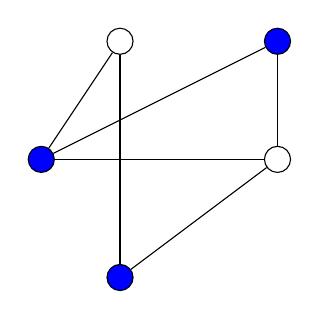
\begin{tikzpicture}[node distance={30mm}, main/.style = {draw, circle}] 
        \node[main] (1) at (4, 2) {}; 
        \node[main, fill=blue] (2) at (6, 2) {};
        \node[main, fill=blue] (3) at (3, 0.5) {};
        \node[main] (4) at (6, 0.5) {};
        \node[main, fill=blue] (5) at (4, -1) {};

        \draw (1) -- (3); \draw (1) -- (5); \draw (2) -- (3);
        \draw (2) -- (4); \draw (3) -- (4); \draw (4) -- (5);
    \end{tikzpicture} 
\end{center}\vspace{-0.25cm}
On the other hand, the complete graph $K_5$ has no vertex cover with size 
at most $\ell = 3$. 

\begin{prop}{prop:6.2}
    \textsc{DecVC} is $\NP$-complete.
\end{prop}\vspace{-0.25cm}
\begin{pf}[Proposition~\ref{prop:6.2}]
    We use the recipe that we supplied above. First, we show 
    that $\textsc{DecVC} \in \NP$. Consider a subset of vertices $U \subseteq V$ 
    to be our certificate. It is easy to verify that $|U| \leq \ell$. We can 
    iterate through the edge set and determine if one of the endpoints 
    is in $U$. Overall, the certifier can be implemented in linear time. 
    
    Now, we reduce a known $\NP$-complete problem to $\textsc{DecVC}$. 
    Here, we only have $\textsc{3-SAT}$ at our disposal, so let's show that 
    $\textsc{3-SAT} \leq_p \textsc{DecVC}$. 

    Suppose that are are given an instance of \textsc{3-SAT}. In particular, 
    we have variables $x_1, \dots, x_n$ and clauses $C_1, \dots, C_k$ 
    of the form $t_1 \vee t_2 \vee t_3$ where $t_1, t_2, t_3 \in 
    \{x_1, \dots, x_n\} \cup \{\overline{x_1}, \dots, \overline{x_n}\}$. 
    We construct an instance of \textsc{DecVC} as follows:
    \begin{itemize}
        \item Let's start with the graph $G = (V, E)$. For every clause 
        $C_i = t_1 \vee t_2 \vee t_3$ where $i = 1, \dots, k$, introduce the 
        vertices $(t_1, i)$, $(t_2, i)$, and $(t_3, i)$. Add edges between 
        each pair of vertices to form a triangle. 

        Next, for each variable $x_j$ appearing in clause $C_{i_1}$ as $x_j$
        and in clause $C_{i_2}$ as $\overline{x_j}$ where $i_1 \neq i_2$, 
        include an edge between $(x_j, i_1)$ and $(\overline{x_j}, i_2)$.
        
        \item Let $\ell = 2k$ be twice the number of clauses.
    \end{itemize}
    Next, we show that the original \textsc{3-SAT} instance is a ``yes'' 
    instance if and only if the constructed \textsc{DecVC} instance 
    is a ``yes'' instance. In particular, if we have an oracle that 
    solves \textsc{DecVC}, then we can also solve \textsc{3-SAT} efficiently. 

    $(\Rightarrow)$ Suppose that the original \textsc{3-SAT} instance 
    is a ``yes'' instance. Then there is some truth assignment $v$ to 
    the variables $x_1, \dots, x_n$ such that $C_1 \wedge \cdots \wedge C_k$ 
    is satisfied. For each clause $C_i = t_1 \vee t_2 \vee t_3$, there exists 
    $t \in \{t_1, t_2, t_3\}$ such that $t = \textsf{True}$ for the assignment 
    $v$. Let $y_i$ denote this $t$ for all $i = 1, \dots, k$. 

    Let $U = V \setminus \{(y_i, i) : i = 1, \dots, k\}$ and observe that 
    $|U| = |V| - k = 3k - k = 2k = \ell$. Moreover, we claim that $U$ is a 
    vertex cover for $G = (V, E)$. Suppose otherwise, so there is some $e \in E$ 
    with both endpoints not in $U$. By construction, these endpoints are 
    $(y_i, i)$ and $(y_j, j)$ for some $i \neq j$. It is clear that 
    this edge is not one from the triangle between $(t_1, i)$, $(t_2, i)$
    and $(t_3, i)$ for a clause $C_i = t_1 \vee t_2 \vee t_3$ since $i \neq j$.
    Moreover, it cannot be an edge between $(x_t, i)$ and $(\overline{x_t}, j)$ 
    for some variable $x_t$ since $v$ would not be a valid truth assignment.
    Therefore, both cases are impossible, so $U$ must be a vertex cover. 
    That is, our constructed \textsc{DecVC} instance is a ``yes'' instance.

    $(\Leftarrow)$ Suppose now that our constructed \textsc{DecVC} instance 
    is a ``yes'' instance. Let $U$ be a vertex cover in $G$ such that 
    $|U| \leq \ell = 2k$. By construction of the graph $G = (V, E)$, 
    it must be the case that $|U| = 2k$ because for each clause 
    $C_i = t_1 \vee t_2 \vee t_3$, the vertex cover must take two 
    out of three of the vertices $(t_1, i)$, $(t_2, i)$, and $(t_3, i)$. 

    Let $(y_i, i)$ be the vertex that is not in $U$ from $y_i \in 
    \{t_1, t_2, t_3\}$. Define an truth assignment $v$ to $x_1, \dots, x_n$ 
    such that $y_i = \textsf{True}$ for all $i = 1, \dots, k$. Suppose that 
    $v$ is not well-defined. That is, there is a variable $x_t$ which 
    needs to be assigned both \textsf{True} and \textsf{False}. 
    Then we have $y_i = x_t$ and $y_j = \overline{x_t}$ for some $i \neq j$. 
    By construction of $G = (V, E)$, there is an edge between $(y_i, i)$ 
    and $(y_j, j)$. Neither of these endpoints are in $U$, which 
    contradicts the fact that $U$ is a vertex cover.

    Therefore, the truth assignment $v$ is well-defined, and it corresponds 
    to satisfying each clause $C_i$. This means that the original 
    \textsc{3-SAT} instance is a ``yes'' instance, as desired. \qed 
\end{pf}\vspace{-0.25cm}
In Section~\ref{sec:5}, we claimed that the Steiner tree problem 
was $\NP$-hard. Let's now prove this. First, we state the 
decision Steiner tree problem, denoted \textsc{DecSteinerTree}. 
We are given a graph $G = (V, E)$, terminals $T \subseteq V$, 
edge costs $c_e \geq 0$ for each $e \in E$, and a number $k$. 
The goal is to determine whether there is a Steiner tree $F \subseteq E$ 
such that $c(F) \leq k$. 

\begin{prop}{prop:6.3}
    \textsc{DecSteinerTree} is $\NP$-complete.
\end{prop}\vspace{-0.25cm}
\begin{pf}[Proposition~\ref{prop:6.3}]
    We see that $\textsc{DecSteinerTree} \in \NP$ by taking a subset 
    $F \subseteq E$ as a certificate. It is easy to check that $c(F) \leq k$
    and that there is a $u, v$-path in $F$ for every $u, v \in T$ in 
    polynomial time. 

    Next, we show that $\textsc{DecVC} \leq_p \textsc{DecSteinerTree}$, 
    where we know that $\textsc{DecVC}$ is $\NP$-complete from 
    Proposition~\ref{prop:6.2}. Suppose that we are given a graph 
    $G = (V, E)$ and a number $\ell$ from $\textsc{DecVC}$. We 
    construct a \textsc{DecSteinerTree} instance as follows: 
    \begin{itemize}
        \item Let $G' = (V', E')$ where $V' = \{r\} \cup V \cup \{t_e : 
        e \in E\}$ and 
        \[ E' = \{rv : v \in V\} \cup \{vt_e : e \in E \text{ and $v$ 
        is an endpoint of $e$}\}. \]
        In particular, we can view the graph $G'$ as one consisting of three 
        ``layers'': one with the new vertex $r$ at the top, the original 
        vertices $V$ in the middle, and new vertices $t_e$ corresponding to 
        each edge $e \in E$ at the bottom. There is an edge from $r$ to 
        each original vertex $v \in V$, and an edge from each $v \in V$ 
        to $t_e$ if $v$ is an endpoint of $e$. 
        \item The terminals will be $T = \{r\} \cup \{t_e : e \in E\}$; namely, 
        the edges in the top and bottom layers.
        \item We assign edge costs via 
        \[ c_e = \begin{cases}
            100|V|, & \text{if } e \in \{vt_e : e \in E \text{ and $v$ 
            is an endpoint of $e$}\}, \\ 
            1, & \text{otherwise.}
        \end{cases} \]
        \item Finally, we set $k = 100|V||E| + \ell$. 
    \end{itemize}\newpage 
    We claim that the original \textsc{DecVC} instance is a ``yes'' instance 
    if and only if the \textsc{DecSteinerTree} instance is a 
    ``yes'' instance. 

    $(\Rightarrow)$ Suppose that the original \textsc{DecVC} instance is a 
    ``yes'' instance. Then there is a vertex cover $U \subseteq V$ 
    of $G = (V, E)$ such that $|U| \leq \ell$. For each $e \in E$, let 
    $u_e \in U$ be a vertex such that $e \in \delta(u_e)$ (when both 
    endpoints are in $U$, we can arbitrarily pick one).

    Consider the set of edges
    $F := \{ru : u \in U\} \cup \{t_e u_e : e \in E\} \subseteq E'$. 
    Note that this has cost 
    $c(F) = |U| + 100|V||E| \leq \ell + 100|V||E| = k$ and that 
    $F$ is a Steiner tree of $G' = (V', E')$ with respect to the 
    terminals $T = \{r\} \cup \{t_e : e \in E\}$, so the \textsc{DecSteinerTree}
    instance is a ``yes'' instance.

    $(\Leftarrow)$ Suppose that the \textsc{DecSteinerTree} instance 
    is a ``yes'' instance. Moreover, towards a contradiction, assume 
    that the original \textsc{DecVC} instance is a ``no'' instance. 
    There exists a Steiner tree $F \subseteq E'$ for $G' = (V', E')$ 
    with respect to $T$ such that $c(F) \leq k = \ell + 100|V||E|$. 

    Let $\overline{E} = \{vt_e : e \in E \text{ and $v$ is an endpoint of $e$}\}$ 
    and observe that 
    \[ c(F \cap \overline{E}) \geq 100|V||E| \] 
    since $100|V|$ is the cost of each edge incident to $t_e$ for $e \in E$, 
    and the number of terminals is $|E|$. This bound together with
    $c(F) \leq \ell + 100|V||E|$ implies that $c(F \setminus \overline{E}) \leq \ell$. 

    We may assume that $\ell \leq |V|$, for otherwise \textsc{DecVC} 
    is always a ``yes'' instance. Every vertex $t_e$ corresponding to $e \in E$ 
    is incident to exactly one edge of $F$, because adding even one 
    extra edge incident to $t_e$ leads to 
    \[ c(F) \geq 100|V||E| + 100|V| > 100|V||E| + \ell = k, \] 
    which is a contradiction. Construct the set 
    \[ U = \{v \in V : v \text{ is an endpoint of an edge in } F \setminus \overline{E}\}. \] 
    Note that $|U| \leq c(F \setminus \overline{E}) \leq \ell$ since 
    each edge from $F \setminus \overline{E}$ has cost $1$. Moreover, 
    $U$ is a vertex cover for the original $\textsc{DecVC}$ instance. 
    Otherwise, there would exist some terminal $t_e$
    such that $t_e$ is adjacent only to $u_e$ in $F$. But $u_e$ 
    is only adjacent to terminals of the form $t_g$ where $g \in E$. 
    This implies that $u_e$ is not connected to $r$, which is a contradiction. \qed
\end{pf}\vspace{-0.25cm}
